\documentclass{standalone}
\usepackage{tikz, ifthen}
\usepackage{amsmath}

\begin{document}

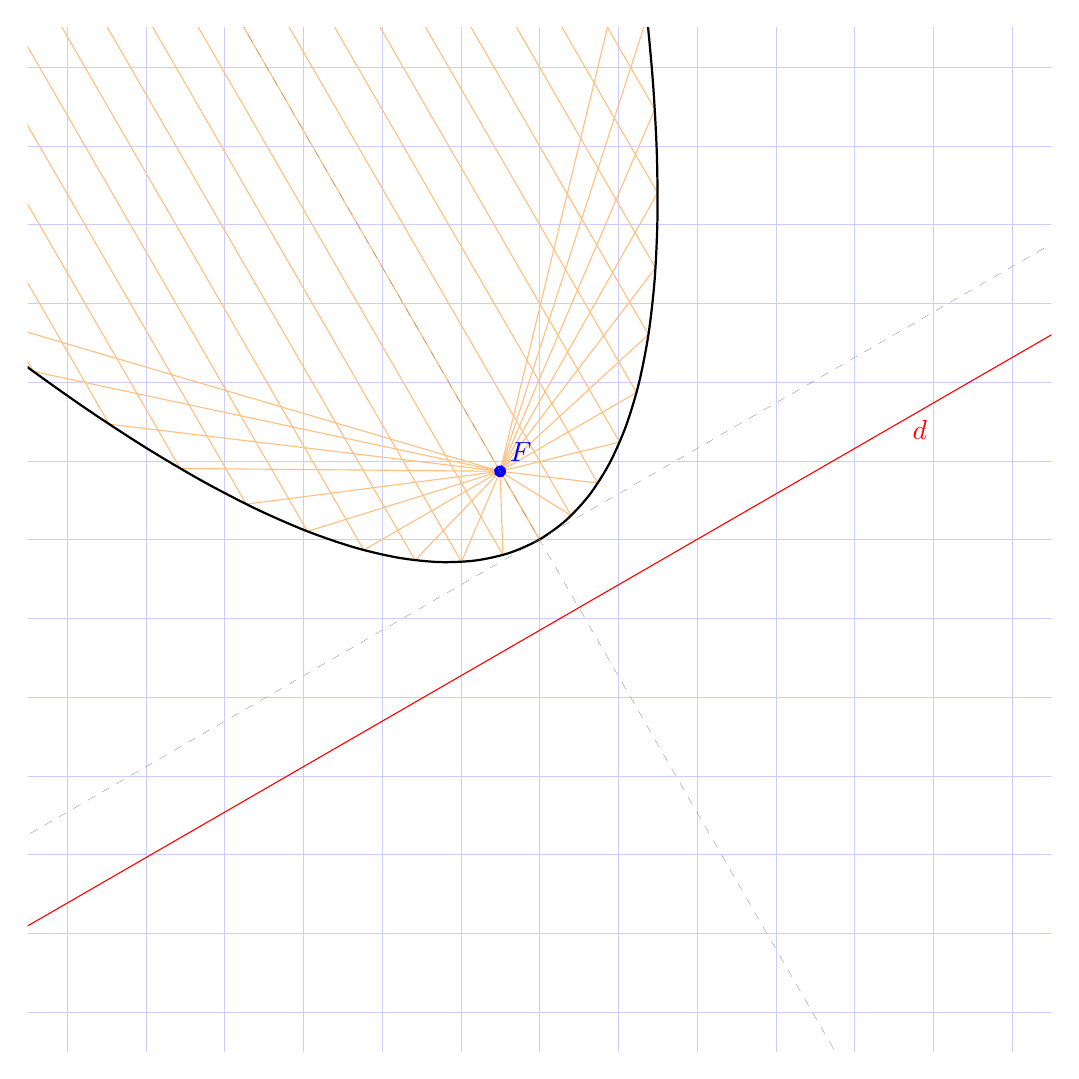
\begin{tikzpicture}
    
    % Center of the circle
    \def\xmin{-6}
    \def\xmax{6}
    \def\ymin{-6}
    \def\ymax{6}
    \def\dx{.5}
    \def\dy{.5}
    \def\xminb{\xmin-\dx}
    \def\xmaxb{\xmax+\dx}
    \def\yminb{\ymin-\dy}
    \def\ymaxb{\ymax+\dy}
    \def\xa{-2}     % x focus A 
    \def\ya{ 0}     % y focus A
    \def\xb{ 2}     % x focus B
    \def\yb{ 0}     % y focus B
    \def\xpmin{-6}
    \def\xpmax{ 6}
    \def\ypmin{-5.5}
    \def\ypmax{ 5.5}
    \def\d{2.};
    \def\a{0.5/\d};
    \coordinate (fa) at (\xa, \ya);
    \coordinate (fb) at (\xb, \yb);
    \def\c{sqrt((\xb-\xa)*(\xb-\xa)+(\ya-\yb)*(\ya-\yb))/2};
    \def\xc{0.5*(\xa+\xb)};
    \def\yc{0.5*(\ya+\yb)};
    \coordinate (center) at ({\xc}, {\yc});
%   \def\b{sqrt(\c*\c-\a*\a)}; % hyperbola
    \def\b{sqrt(\a*\a-\c*\c)}; % ellipses
%   \def\alpha{{atan2(\yb-\ya,\xb-\xa)}};
    \def\alpha{30}

    \clip (\xminb, \yminb) rectangle (\xmaxb, \ymaxb);

    % Draw grid
    \draw[step=1., blue!20, ultra thin] (\xmin-2, \ymin-2) grid (\xmax+2, \ymax+2); % Visible grid with lighter color

%   % Axes, x
%   \draw[->, thick, blue] (\xmin, 0) -- (\xmax, 0) node[below right] {$x$};
%   \draw[    thick, blue] (\xmin-2, 0) -- (\xmax+2, 0);
%   \draw[->, thick, blue] (0, \ymin) -- (0, \ymax) node[right] {$y$};
%   \draw[    thick, blue] (0, \ymin-2) -- (0, \ymax+2);
%   % Axis ticks
%   \foreach \x in {\xmin,..., \xmax}{
%       \ifthenelse{ \x = 0 }{}{\draw[blue] (\x, -0.1) -- (\x, +0.1) node[below=8pt, left=0pt] {\small $\x$};}
%   }
%   \foreach \y in {\ymin,..., \ymax}{
%       \ifthenelse{ \y = 0 }{}{\draw[blue] (-0.1, \y) -- (0.1, \y) node[left=4pt] {\small $\y$};}
%   }

    % Rays
    \foreach \x in {-10,...,10}{
        \draw[orange!50, thin, rotate=\alpha] ({\x/2}, {2*\ymax}) -- ({\x/2},{\a*\x/2*\x/2});
        \draw[orange!50, thin, rotate=\alpha] (0,{\d/2}) -- ({\x/2},{\a*\x/2*\x/2});
    }
    
    % Parabola
    \draw[thick, black, rotate=\alpha] plot[parametric, smooth, domain=-5:5] ({\xc+\x}, {\yc+\a*\x*\x});
    % Focus
    \filldraw[blue, rotate=\alpha] (0,{\d/2}) circle (2pt) node[above right] {$F$};
    % Directrix
    \draw[red, rotate=\alpha] (-10,{-\d/2}) -- (10,{-\d/2});
    \filldraw[red, rotate=\alpha] (5,-1) circle (0) node[below] {$d$};

    % Construction lines
    \draw[ultra thin, black!50, dashed, rotate=\alpha] (0,-10) -- (0,10);
    \draw[ultra thin, black!50, dashed, rotate=\alpha] (-10,0) -- (10,0);

\end{tikzpicture}

\end{document}
